\section{انواع مدل های استفاده شده}

در این بخش  به انواع مدل های استفاده شده در کد اشاره میکنیم و هر کدام را به صورت خلاصه توضیح میدهیم. 

تمامی مدل هایی که مورد بررسی قرار میگیرند در زیر آورده شده و هر کدام به صورت کوتاه توضیح داده میشوند. 

\begin{enumerate}
	\item 
	\lr{\textbf{Logistic Regression}}
	
	این مدل یک دسته‌بند 2 تایی است. این مدل به این صورت عمل میکند که ابتدا یک لایه خطی روی ورودی ها اعمال کرده و سپس خروجی را از تابع $sigmoid$ که به صورت 
	$f(x) = \frac{1}{1 + e^{-x}}$
	تعریف میشود، عبور میدهد. این تابع به نوعی محور اعداد را به بازه 
	$[0, 1]$
	تبدیل کرده و $Squish$ میکند. شکل تابع $sigmoid$ را میتوانید در شکل زیر ببینید:
	
	\begin{figure}[h]
		\centering
		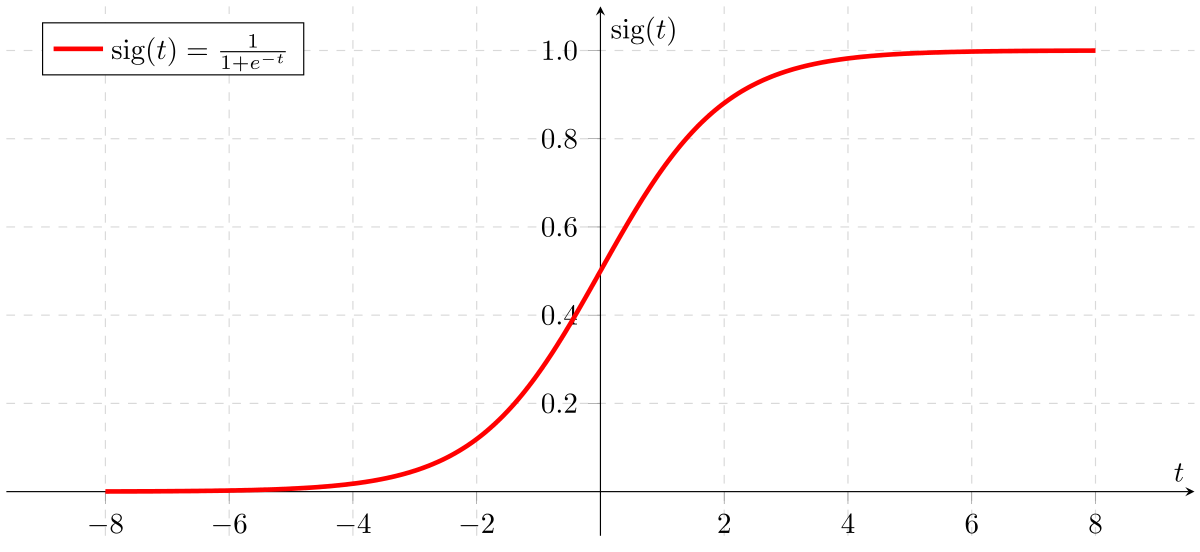
\includegraphics[width=0.6\textwidth]{training/2}
		\caption{تابع \lr{sigmoid}}
		\label{fig:training:sigmoid}
	\end{figure} 
	
	
	سپس در نهایت با توجه به اینکه خروجی‌ مان بیش از $\frac{1}{2}$ است یا نه به یکی از 2 دسته تعلق میگیرد. مدل را در شکل زیر میتوان به صورت خلاصه دید:
	
	\begin{figure}[h]
		\centering
		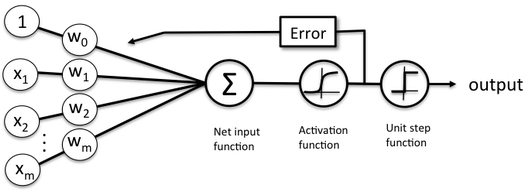
\includegraphics[width=0.6\textwidth]{training/1}
		\caption{مدل \lr{Logistic Regression}}
		\label{fig:training:logisitic-regression}
	\end{figure} \pagebreak
	
		
	\item 
	\lr{SVM}
	
	این مدل نیز مشابه مدل قبل، یک دسته‌بند 2 تایی میباشد. هدف این مدل این است که به نوعی خطی از بین داده های 2 کلاس طوری انتخاب کند که اولا داده های هر کلاس یک طرف خط قرار بگیرند و ثانیا فاصله بین نزدیکترین داده ها تا این خط، ماکسیمم باشد. یعنی درواقع \lr{margin} خطا تا حد امکان بیشینه باشد. 
	
	\begin{figure}[h]
		\centering
		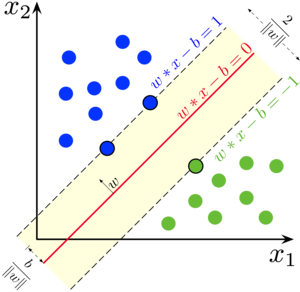
\includegraphics[width=0.4\textwidth]{training/3}
		\caption{مدل \lr{SVM}}
		\label{fig:training:svm}
	\end{figure}

	ممکن است در ابتدا، این هدف کمی عجیب بنظر بیاید. اما دلیل آن این است که اگر ورودی هایی که میخواهیم در آینده به مدل بدهیم را نقاطی در فضا در نظر بگیریم، با ماکسیمم کردن این $margin$ به نوعی داریم امکان دسته‌بندی شدن اشتباه را کمینه میکنیم با این فرض که نقاط مربوط به هر کلاس نزدیک هم قرار دارند. 
	
	
	
	\item 
	\lr{Decision Tree \& Random Forest}
	
	این مدل برخلاف مدل های قبلی، امکان دسته‌بندی چند کلاسه را به طور مستقیم را دارد. از بین تمامی مدل ها، اینها آشناترین و راحت ترین مدل ها برای فهم انسان ها میباشند. نحوه عملکرد آنها این است که درختی از تصمیم های متوالی تولید میکنند و به ازای هر ورودی، این درخت را پیمایش کرده تا به یک برگ برسند و در کلاس مربوط به آن برگ را خروجی میدهند. 
	
	\begin{figure}[h]
		\centering
		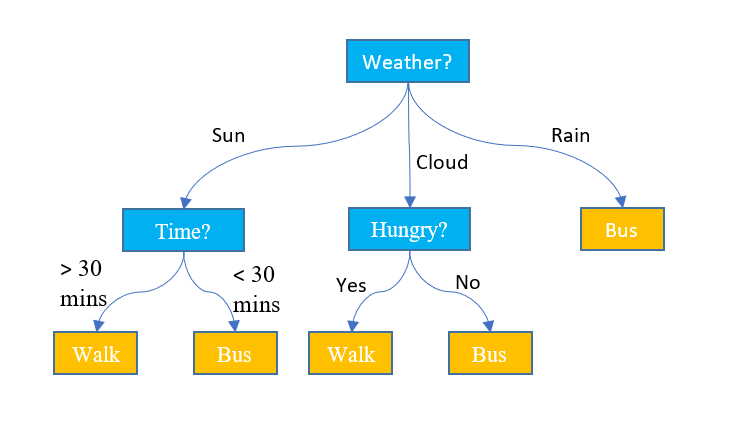
\includegraphics[width=0.6\textwidth]{training/4}
		\caption{مدل درخت تصمیم (\lr{Decision Tree})}
		\label{fig:training:decision-tree}
	\end{figure}
	
	گرچه این مدل ها، شکل کلی ساده‌ای دارند، اما یک بدی آنها این است که خیلی قابلیت $overfit$ شدن دارند. به این معنا که درختی که میسازند، ممکن است زیادی به داده ورودی مرتبط باشد و به جزئیات غیر مربوط به کلاسی که داریم دسته‌بندی میکنیم، توجه کند و بر اساس آنها تصمیم بگیرد. این مشکل را تا حدی با معرفی مدل های 
	\lr{Random Forest}
	برطرف میکنند. در این مدل ها، به جای 1 درخت، چندین درخت (یک جنگل) ساخته شده و در نهایت از آنها استفاده میشود. با انجام اینکار با رعایت کردن نکاتی در هنگام آموزش، میتوانیم تا حدی مشکل $overfitting$ درخت های تصمیم را کاهش بدهیم.
	
	\item 
	\lr{Gradient Boosting}
	
	این روش، در واقع یک مدل نیست بلکه روشی است برای سوار کردن تعدادی مدل ساده روی هم به این امید که مجموع آنها، مدلی دقیق و قوی به ما بدهد. شکل کلی این روش به این صورت است که تعدادی مدل ساده یاد گرفته میشود. سپس داده هایی که به وسیله این مدل های ساده، هنوز اشتباه دسته‌بندی میشوند، را با وزن بیشتر و داده هایی که صحیح دسته‌بندی میشوند را با وزن کمتر در نظر میگیریم و دوباره مدلی برای این داده های جدید بدست می آوریم. در واقع در هر مرحله، سعی میکنیم مدل این مرحله‌مان، تا حد ممکن، ضعف های مدل های قبلی را جبران کند. 
	
	\item 
	\lr{Multi Layer Perceptron (Neural Network)}
	
	این مدل ،آخرین مدل های استفاده شده است. این مدل نوع خاصی از دسته بزرگتری از مدل ها است که به آنها شبکه های عصبی میگویند. میتوان این مدل را گسترشی از مدل \lr{Logistic Regression} در نظر گرفت به این صورت که در آن مدل، یک لایه خطی استفاده میشد و روی آن تابع $sigmoid$ زده میشد. اما در اینجا، چندین لایه داریم و در نهایت یک یا چند خروجی میتوانیم داشته باشیم. مشابه قبل، هر لایه، یک تبدیل خطی روی ورودی های لایه است که بعد از آن، هر کدام از تابع $sigmoid$ رد میشوند و به عنوان ورودی لایه بعدی داده میشوند. 
	
	شمایی  کلی از آنها را میتوان در شکل زیر دید:
	\begin{figure}[h]
		\centering
		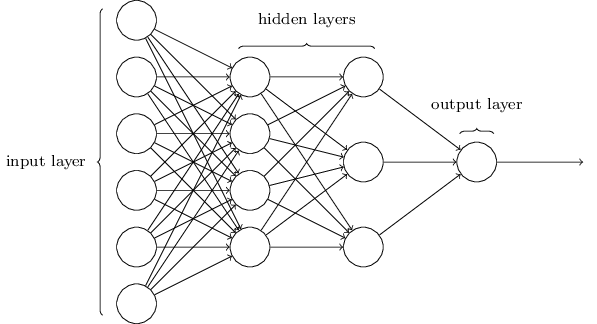
\includegraphics[width=0.6\textwidth]{training/5}
		\caption{مدل (\lr{MLP})}
		\label{fig:training:mlp}
	\end{figure} \pagebreak

\end{enumerate}

